\subsection{BP 6
  Solitary wave on a conical island (Laboratory)}

{\bf Documentation:}
\begin {itemize}

\item \cite{bp-description}
\item \url{http://chl.erdc.usace.army.mil/chl.aspx?p=s&a=Projects;35}
\item PMEL-135, pp 6 \& 39-45 \cite{SynolakisBernard:pmel135}.
\item Other reference, below
\end{itemize} 

\subsubsection {Problems encountered}

\begin {itemize}
\item Details of the laboratory setup and, therefore, the computational domain could not not be determined by the available documentation.  In particular, the following items were not documented: (a) the distance from the wavemaker face to the island center and (b) open gaps at each end of the wavemaker.
\item Erroneous entries were found in data files ts2a.txt, ts2b.txt and ts2cnew1.txt.  Several entries of the letter "M" triggered read-in error messages; they were replaced by linear interpolation or extrapolation of neighboring values.
\end{itemize} 

\subsubsection{What we did}

\begin{itemize}
\item Used $g=9.81$ and no friction.
\item Used the computational domain presented in \Fig{bp6/Domain.pdf}, developed after personal communication with Michael Briggs, U.S. Army Corps of Engineers, who  provided additional information on physical details of the laboratory experiment.
\item Used open boundary conditions for the top, bottom and right walls, and for the gaps between the ends of the wavemaker and the top and bottom walls.
\item Used boundary conditions for the face of the wavemaker at the left wall corresponding to the ...  
\item Simulated Cases A and C, each with three different grid sizes and resolution, to demonstrate convergence:  61 X 47 (50 cm), 121 X 93 (25 cm) and 241 X 185 (12.5 cm)
\end{itemize}

\subsubsection{Results}


{\bf References:}
\begin {itemize}

\item briggs1:  Briggs, M.J., Synolakis, C.E., Harkins, G.S. (1994):  Tsunami runup on a conical island.  Proc. of Waves — Physical and Numerical Modelling, 21-24 August 1994, Vancouver, Canada, V1, 446-455.
\item Briggs, M.J., C.E. Synolakis, G.S. Harkins, and D. Green (1995): Laboratory experiments of tsunami runup on a circular island. Pure Appl. Geophys., 144, 569-593.
\item Briggs, M.J., C.E. Synolakis, G.S. Harkins, and D. R. Green (1996): Runup of solitary waves on a circular island, in Proceedings of the Second International Long-Wave Runup Models, Friday Harbor, Washington, 12-16 September 1995, 363-374.
\item Liu, P.L.-F., Y.-S. Cho, K. Fujima (1994):  Numerical Solutions of Three-Dimensional Run-up on a Circular Island, 21-24 August 1994, Vancouver, Canada, V2, 1031-1040.
\item Liu, P.L.-F., Y.-S. Cho, M.J. Briggs, U. Kânoglu, and C.E. Synolakis (1995): Runup of solitary waves on a circular island. J. Fluid Mech., 302, 259-285.
\item Yeh, H., P. Liu, M. Briggs, C. Synolakis, (1994): Propagation and amplification of tsunamis at coastal boundaries, Nature 372, 353-355.
\end{itemize}

\begin{figure}[ht]
\hfil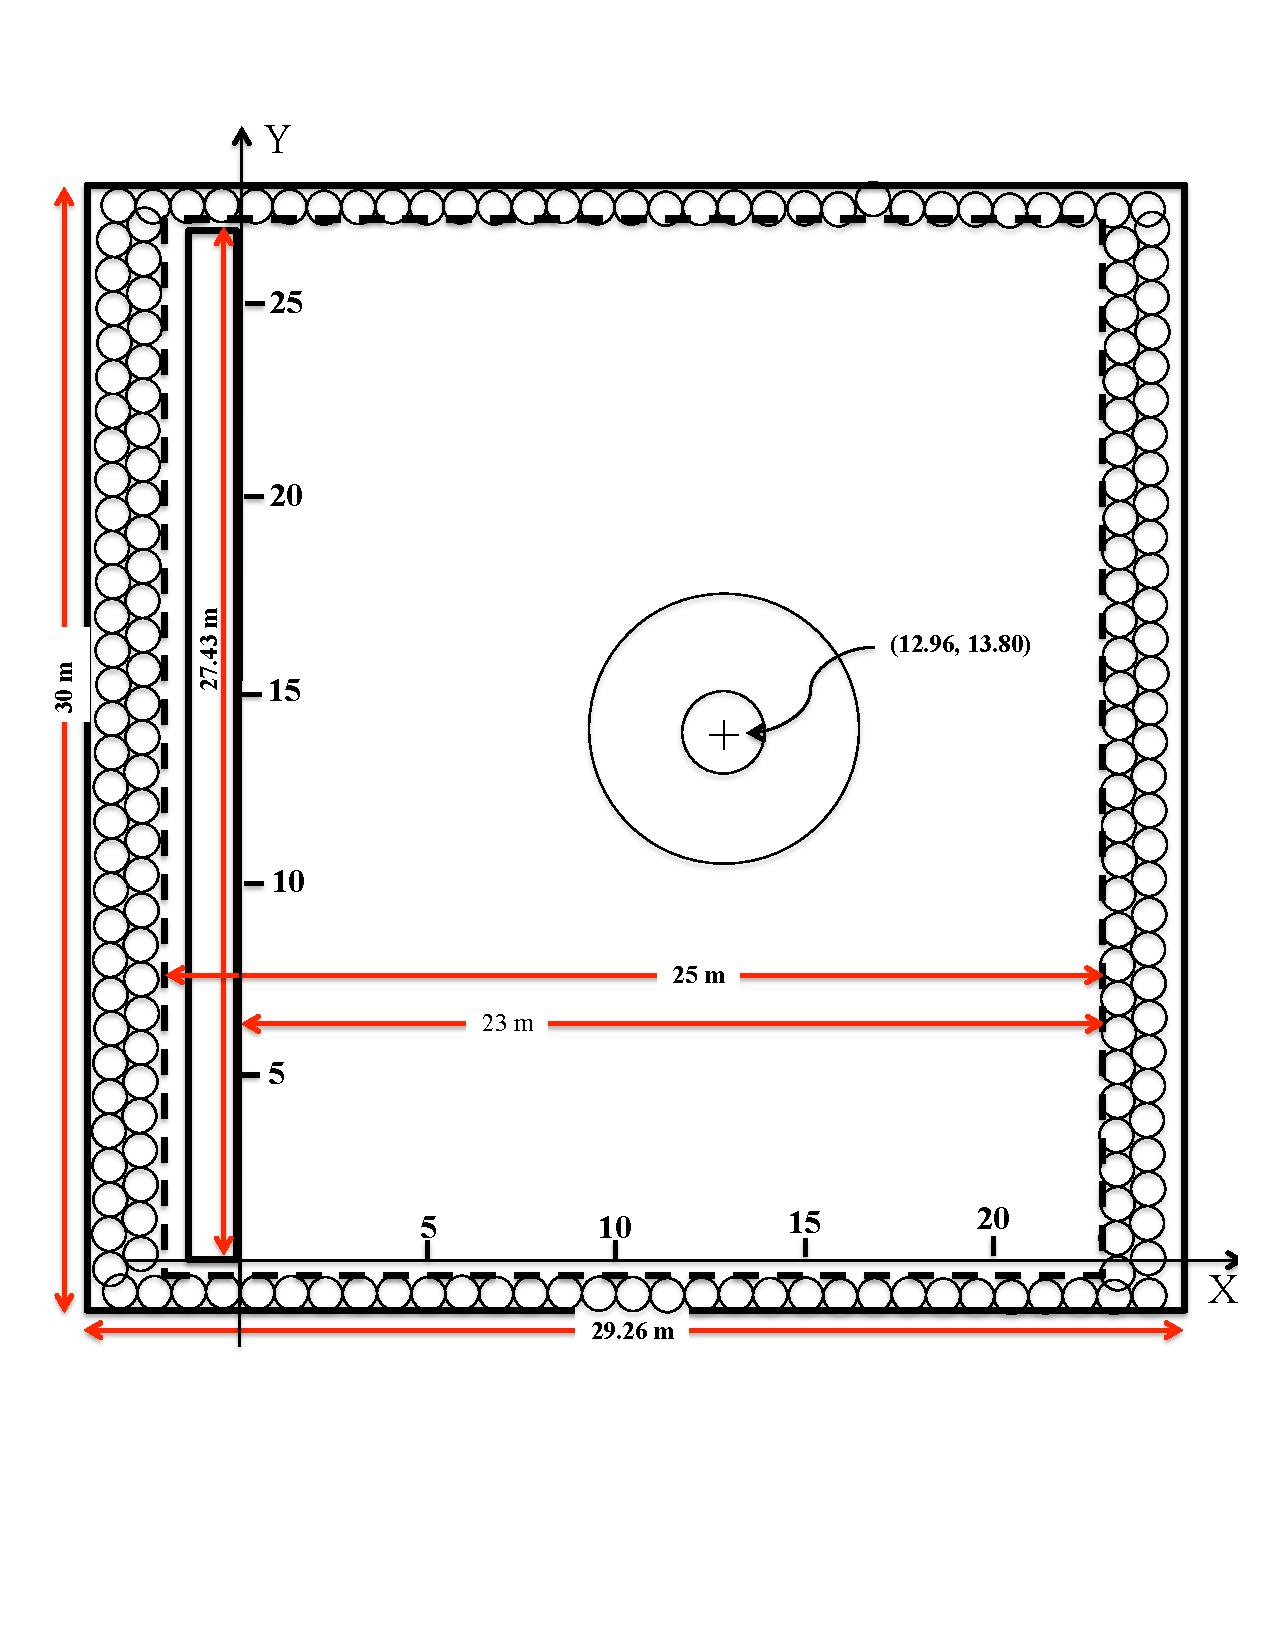
\includegraphics[width=1.5in]{bp6/Domain.pdf}\hfil
\end{figure}

\todo{Move these to references.bib}
